% =====================================================================
% DhyutimaanPI — CAISc 2026 Submission
% Track: Verifiable
% =====================================================================
\documentclass{article}
\PassOptionsToPackage{numbers,compress}{natbib}
\usepackage{caisc_2026}
\usepackage[utf8]{inputenc}
\usepackage[T1]{fontenc}
\usepackage{hyperref}
\usepackage{url}
\usepackage{booktabs}
\usepackage{amsfonts}
\usepackage{amsmath}
\usepackage{amssymb}
\usepackage{nicefrac}
\usepackage{microtype}
\usepackage[table]{xcolor}
\usepackage{colortbl}
\usepackage{graphicx}
\usepackage{multirow}
\usepackage{array}

% ── Convenience macros ───────────────────────────────────────────────
\newcommand{\dhyutimaan}{\textsc{DhyutimaanPI}}
\newcommand{\Ltwo}{L^2}
\newcommand{\relL}{\varepsilon_{\mathrm{rel}}}
\newcommand{\bfx}{\mathbf{x}}

% ── Title ─────────────────────────────────────────────────────────────
\title{\dhyutimaan: An Agentic Pipeline for Reproducible\\
       PINN Failure-Mode Discovery via Systematic\\
       Factorial Experimentation}

\author{%
  Rahul Sundar\\
  \texttt{rahul.sundar95@gmail.com}
}

\begin{document}
\maketitle

% ─────────────────────────────────────────────────────────────────────
\begin{abstract}
Recommended PINN training strategies — hard-constraint output transforms,
causal temporal weighting, L-BFGS polishing, Fourier-feature encodings —
are each well-motivated by theory and validated on specific problem classes
in the literature.
Yet when a practitioner applies them to a new problem, failures can be
\emph{silent}: training loss converges, runs appear successful, but the
solution field is wrong.
Detecting such failures requires more than monitoring loss curves; it requires
a reproducible experimental infrastructure with pre-registered falsifiable
hypotheses, systematic multi-factor comparisons, and per-region adversarial
error auditing.

We present \dhyutimaan{}, a four-skill agentic pipeline that provides exactly
this infrastructure.
It automates the full PINN research workflow — literature survey, problem
specification, code generation, experiment execution, and adversarial
post-training analysis — through a chain of composable skills connected
by stable machine-readable artefacts.
The critical component is the \emph{Analyst} skill, whose diagnostic posture
treats a converged training loss as a necessary but not sufficient condition
for accuracy, and mandates per-time-slice and per-region error evaluation
against an exact reference.

We demonstrate the framework on a $2^3$ full-factorial design of experiments
across 26 variants: 16 on steady and unsteady 2D heat conduction, 8 on
1D viscous Burgers at $\nu = 0.01/\pi$, and 2 viscosity stress tests
at $\nu\in\{0.001/\pi,\,0.1/\pi\}$.
Nine of ten pre-registered hypotheses are refuted; one is confirmed.
More importantly, three variants exhibit converged training losses while
producing solution errors of \emph{order unity} — failures invisible from
loss curves alone and detectable only through \dhyutimaan{}'s systematic
per-slice verification.
Specifically, causal temporal weighting~\citep{wang2022causal} — effective
on stiff and advection-dominated problems — produces relative $L^2$ error of
$0.89$ ($367\times$ growth) when applied to a smooth parabolic solution
outside its validated regime, versus $8.7\times10^{-4}$ for the
hard-constraint standard baseline.
Analytical derivations explain (i) the causal weight starvation mechanism
responsible for this failure; (ii) why the hard-constraint parabolic ansatz
is in fact regular at $t=0$, contradicting the singularity hypothesis; and
(iii) why a finite-difference Laplacian eliminates gradient signal when
backpropagated through an MLP — a silent implementation pathology.
\dhyutimaan{}'s per-slice verification is what makes these failures \emph{detectable};
its pre-registered hypotheses and traceable artefact architecture are what make them
\emph{attributable} --- every quantitative claim is linked to a specific variant, file,
and mechanism --- rather than anecdotal.
\end{abstract}

% ─────────────────────────────────────────────────────────────────────
\section{Introduction}
\label{sec:intro}

Physics-Informed Neural Networks (PINNs)~\citep{raissi2019} encode governing
equations as residual constraints in a neural network objective, enabling
mesh-free solution of forward and inverse problems across continuum mechanics.
The field has accumulated a rich toolkit of training interventions:
hard-constraint output transforms that embed boundary conditions
exactly~\citep{lagaris1998}, adaptive loss-balancing
schemes~\citep{wang2021gradpath,bischof2021relobralo}, causal temporal
weighting for time-dependent problems~\citep{wang2022causal}, and
Fourier-feature encodings that overcome spectral
bias~\citep{tancik2020ff,wang2021ntk}.
Each intervention is supported by sound motivation and demonstrated benefit
on at least one benchmark problem.

\paragraph{The reproducibility gap.}
Despite this theoretical grounding, a practitioner applying these techniques
to a new problem faces a structural hazard: \emph{training loss convergence
does not certify solution accuracy}.
An optimiser can converge on a function that satisfies the sampled collocation
residuals while failing badly in unseen regions, at later times, or near
boundary layers.
The existing literature largely reports results on the problems where each
technique was designed to succeed; failure modes on out-of-design problems
are rarely documented, and when they occur they are often not detected because
evaluation is limited to monitoring aggregate training loss.

This gap is not a flaw in individual papers — it reflects the challenge of
a prevalent experimental practice: reporting on benchmarks where each
intervention was designed to succeed, with evaluation limited to aggregate
training loss.
Without pre-registered falsifiable hypotheses there is no criterion for
refutation; without per-region verification there is no mechanism to
distinguish a converged loss from a converged solution.

\paragraph{\dhyutimaan{}.}
We present \dhyutimaan{} (\textit{Dhyutimaan}, Sanskrit: \textit{luminous,
radiant}), a four-skill agentic pipeline that closes this gap by encoding
the PINN research workflow as a reproducible, falsifiable experimental
protocol.
Its four stages — Surveyor, Framer, Implementer, and Analyst — are
connected by stable machine-readable artefacts that constitute explicit
inter-skill contracts.
The Framer enforces pre-registration: every hypothesis must specify an
intervention, a metric, and a threshold before any experiment runs.
The Analyst enforces adversarial verification: per-time-slice and
per-region errors are evaluated against an exact reference, and a
converged training loss is treated as a necessary but not sufficient
condition for declaring a run successful.

\paragraph{What reproducibility reveals.}
Applying \dhyutimaan{} to a $2^3$ factorial DoE on 2D heat conduction
(16 variants) and 1D viscous Burgers (8 variants plus 2 viscosity stress tests)
produces a concrete demonstration of the value of this infrastructure.
Three of the 24 DoE variants exhibit converged training losses but solution
errors of order unity — failures that would be declared successes under
standard loss-curve monitoring.
Nine of ten pre-registered hypotheses are refuted; one is confirmed.
Each refutation exposes a precise mechanistic boundary between problem classes
where a given technique helps and those where it harms; the single confirmation
(Burgers H5: low-viscosity failure at $\nu=0.001/\pi$) demonstrates that the
framework can also reliably \emph{detect} a predicted regime transition that
aggregate metrics would miss.
Causal temporal weighting~\citep{wang2022causal}, effective on stiff
time-dependent problems, produces $367\times$ error growth when applied
to a smooth parabolic solution outside its validated regime — a finding
made possible, and made \emph{attributable}, only by the Analyst's
per-slice verification protocol.

\paragraph{Contributions.}
\begin{enumerate}
  \item The \dhyutimaan{} four-skill pipeline with a formally defined artefact
        schema (Section~\ref{sec:framework}).
  \item A complete, fully reproducible $2^3$ DoE on 2D heat conduction (16
        variants, 20\,000 Adam steps each), with quantitative verdicts on five
        pre-registered falsifiable hypotheses (Section~\ref{sec:heat}).
  \item A complete $2^3$ DoE on 1D viscous Burgers (8 variants, 30\,000 Adam
        steps each), plus two viscosity stress tests, characterising the
        causal-weighting failure regime for solutions developing steep interior
        layers and confirming the only hypothesis in the study (Burgers H5,
        $\nu=0.001/\pi$ causes failure; Section~\ref{sec:burgers}).
  \item Analytical derivations of three failure mechanisms: FD Laplacian
        gradient starvation, causal weight starvation on smooth parabolic
        solutions, and the non-singularity of the parabolic hard-constraint
        ansatz (Appendix~\ref{app:analytics}).
\end{enumerate}

% ─────────────────────────────────────────────────────────────────────
\section{Related Work}
\label{sec:related}

\paragraph{Gradient pathologies in PINN training.}
Wang et al.~\citep{wang2021gradpath} demonstrated that the back-propagated
gradient of the PDE residual loss typically dominates the boundary-condition
gradient by orders of magnitude during early training, and proposed a
learning-rate annealing scheme to restore balance.
Wang et al.~\citep{wang2021ntk} derived the Neural Tangent Kernel (NTK)
governing PINN convergence and showed that training rates are determined by
NTK eigenvalues, providing a theoretical basis for loss-balancing interventions.
Bischof and Kraus~\citep{bischof2021relobralo} introduced ReLoBRaLo, a
single-backward-pass relative loss balancer that achieves faster convergence
than learning-rate annealing on Burgers benchmarks.

\paragraph{Hard-constraint output transforms.}
Lagaris et al.~\citep{lagaris1998} introduced output-transformation ansatze
that enforce Dirichlet boundary conditions exactly, eliminating the boundary
loss term and converting multi-objective optimisation to a single-objective
PDE residual problem.
This approach is standard in the DeepXDE library~\citep{lu2021deepxde} and is
broadly adopted for homogeneous Dirichlet problems.

\paragraph{Causal temporal weighting.}
Wang et al.~\citep{wang2022causal} showed that standard PINNs violate physical
causality — fitting late-time data before early-time residuals have converged
— and proposed a scheme in which the weight assigned to each temporal slab
depends exponentially on the accumulated residual of all preceding slabs.
This has become the state of the art for stiff and advection-dominated
time-dependent problems.
The present work establishes the complementary failure regime, documented
analytically in Appendix~\ref{app:causal_starvation}.

\paragraph{Architectural representations.}
Tancik et al.~\citep{tancik2020ff} demonstrated that random Fourier feature
mappings overcome spectral bias by flattening the NTK eigenspectrum.
Wang et al.~\citep{wang2024pirate} introduced PirateNets, residual adaptive
networks that progressively deepen during training, achieving state-of-the-art
accuracy across a diverse set of PDE benchmarks.

\paragraph{Systematic evaluation.}
Hao et al.~\citep{pinnacle2024} presented PINNacle, evaluating standard PINNs
on over 20 PDEs at NeurIPS 2024 and finding that only 10 of 22 tasks are
solved reliably without architectural intervention.
PINNacle represents the closest prior effort at systematic, multi-problem
evaluation of PINN failure modes.
The present work differs in emphasis rather than intent: where PINNacle
prioritises breadth of PDE coverage, \dhyutimaan{} prioritises pre-registered
falsifiable hypotheses and adversarial per-slice verification as the
methodological core, applied to a small but fully reproducible factorial design
with unit-domain manufactured solutions and analytically known reference solutions.

% ─────────────────────────────────────────────────────────────────────
\section{The \dhyutimaan{} Framework}
\label{sec:framework}

\dhyutimaan{} comprises four specialised skills, each implemented as a
prompt-governed agent with file-system read/write access.
The pipeline is summarised in Table~\ref{tab:pipeline}.

\begin{table}[h]
\centering
\caption{The four-skill \dhyutimaan{} pipeline.}
\label{tab:pipeline}
\small
\begin{tabular}{llp{5.5cm}}
\toprule
Skill & Input artefact & Output artefact \\
\midrule
\textbf{Surveyor}     & User query + web search
                      & \texttt{pinn-knowledge-base.md} \\
\textbf{Framer}       & \texttt{pinn-knowledge-base.md}
                      & \texttt{problem-spec.md} \\
\textbf{Implementer}  & \texttt{problem-spec.md}
                      & \texttt{pinn\_run/} (Python module set) \\
\textbf{Analyst}      & \texttt{training\_log.csv},
                        \texttt{verification.json}
                      & \texttt{analysis-report.md} \\
\bottomrule
\end{tabular}
\end{table}

\paragraph{Surveyor.}
Queries arXiv, Semantic Scholar, and journal repositories for PINN variants
and documented failure modes relevant to the target PDE class.
Synthesises findings into a structured knowledge base with a failure-mode
taxonomy and a ``recommended starting points'' section that the Framer
directly consumes as input context.

\paragraph{Framer.}
Reads the knowledge base and the user's problem description.
Produces a \texttt{problem-spec.md} document containing: (i) governing
equations in mathematical notation; (ii) domain, boundary conditions, and
initial conditions; (iii) reference solution strategy; (iv) a full-factorial
DoE table with explicit variant labels; (v) \emph{falsifiable} hypotheses
each specifying an intervention, a measurement metric, and a quantitative
confirmation threshold; and (vi) anticipated failure modes and their
diagnostic signals.

\paragraph{Implementer.}
Generates a self-contained PyTorch module set: \texttt{problem.py}
(automatic-differentiation PDE residuals, hard-constraint ansatze,
collocation point samplers), \texttt{model.py} (plain tanh MLP and
random Fourier-feature MLP), \texttt{train.py} (Adam with cosine learning-rate
annealing, per-component CSV logging, periodic collocation resampling, optional
L-BFGS polishing), \texttt{verify.py} (relative $L^2$ error evaluation,
per-time-slice error reporting, hypothesis verdict writer), and \texttt{run.py}
(single-command orchestration via a \texttt{--variant} argument).
All PDE residuals use \texttt{torch.autograd.grad} with
\texttt{create\_graph=True} rather than finite-difference approximations
(see Appendix~\ref{app:fd_pathology} for the rationale).

\paragraph{Analyst.}
Loads all \texttt{verification.json} and \texttt{training\_log.csv} files,
computes training-dynamics statistics programmatically, and produces an
adversarial \texttt{analysis-report.md}.
The Analyst's diagnostic posture is explicitly sceptical: a low training loss
is treated as a necessary but insufficient condition for solution accuracy.
The skill mandates auditing each pre-specified failure mode and requires
that every quantitative claim be traceable to a row in an input file.

\paragraph{Artefact schema as contract.}
The stability of filenames and key names across pipeline stages means that
any individual skill can be re-run or upgraded independently.
The Analyst can be improved without re-running experiments; the Implementer
can be replaced with a DeepXDE or JAX backend without modifying the Framer.
This modularity enables controlled A/B testing of individual pipeline
components.

% ─────────────────────────────────────────────────────────────────────
\section{Experiment 1: 2D Heat Conduction}
\label{sec:heat}

\subsection{Problem Setup}

We study two sub-problems on the unit square $\Omega = (0,1)^2$:

\textbf{Problem A (steady Poisson).}
\begin{equation}
  -\Delta u = 2\pi^2 \sin(\pi x)\sin(\pi y), \quad (x,y)\in\Omega, \qquad
  u = 0 \text{ on } \partial\Omega.
\label{eq:prob_A}
\end{equation}
The exact solution is $u_{\rm ref}(x,y) = \sin(\pi x)\sin(\pi y)$.

\textbf{Problem B (unsteady parabolic).}
\begin{equation}
  u_t - \alpha\,\Delta u = 0 \text{ on } \Omega\times[0,T], \qquad
  u(\cdot,\cdot,0) = \sin(\pi x)\sin(\pi y), \qquad
  u = 0 \text{ on } \partial\Omega\times[0,T],
\label{eq:prob_B}
\end{equation}
with $\alpha=1$ and $T=0.1$.
The exact solution is $u_{\rm ref}(x,y,t) = \sin(\pi x)\sin(\pi y)\,e^{-2\pi^2\alpha t}$.

\paragraph{Design of experiments.}
A $2^3$ full-factorial design spans three binary factors:
\textbf{F1} (hard vs.\ soft boundary-condition enforcement);
\textbf{F2} (L-BFGS polishing vs.\ Adam-only for Problem~A;
causal temporal weighting vs.\ uniform for Problem~B);
\textbf{F3} (Fourier-feature input encoding vs.\ plain coordinates).
This yields 8 variants per sub-problem, 16 in total.

\paragraph{Training protocol.}
All variants train for 20\,000 Adam steps with a cosine learning-rate schedule
from $10^{-3}$ to $10^{-5}$ and collocation resampling every 2\,000 steps.
L-BFGS variants receive an additional 500 polishing steps.
The network architecture is a 4-hidden-layer tanh MLP of width 64 for both
sub-problems.
All experiments were executed on an Apple M-series processor using PyTorch's
MPS backend via the \texttt{torchmps} conda environment.
The hard-constraint ansatze are:
\begin{align}
  \hat{u}^A(x,y)    &= x(1{-}x)\,y(1{-}y)\cdot\mathrm{NN}(x,y;\theta), \label{eq:hard_A}\\
  \hat{u}^B(x,y,t)  &= \sin(\pi x)\sin(\pi y)
                       + t\,x(1{-}x)\,y(1{-}y)\cdot\mathrm{NN}(x,y,t;\theta). \label{eq:hard_B}
\end{align}
Causal weighting for Problem~B uses $\varepsilon=100$ and $K=50$ temporal
slabs~\citep{wang2022causal}.

\subsection{Results}

\begin{table}[h]
\centering
\caption{Problem~A (2D steady Poisson): relative $L^2$ error for all eight variants.
Hard-constraint variants (upper block) uniformly achieve $\relL < 5\times10^{-6}$,
more than an order of magnitude below the best soft-constraint variant.}
\label{tab:heat_A}
\small
\begin{tabular}{llllr}
\toprule
Variant & F1 & F2 & F3 & $\relL$ \\
\midrule
hard-lbfgs-ff & Hard & L-BFGS & FF   & $2.14\times10^{-6}$ \\
hard-adam-ff  & Hard & Adam   & FF   & $3.70\times10^{-6}$ \\
hard-adam     & Hard & Adam   & ---  & $4.31\times10^{-6}$ \\
hard-lbfgs    & Hard & L-BFGS & ---  & $4.38\times10^{-6}$ \\
\midrule
soft-lbfgs    & Soft & L-BFGS & ---  & $6.85\times10^{-5}$ \\
soft-adam     & Soft & Adam   & ---  & $2.47\times10^{-4}$ \\
soft-lbfgs-ff & Soft & L-BFGS & FF   & $4.54\times10^{-4}$ \\
soft-adam-ff  & Soft & Adam   & FF   & $5.55\times10^{-4}$ \\
\bottomrule
\end{tabular}
\end{table}

\begin{table}[h]
\centering
\caption{Problem~B (2D unsteady heat): global relative $L^2$ error and per-slice
errors at selected time levels.
Variants exhibiting catastrophic failure ($\relL > 10^{-1}$) are shaded.
The growth ratio is reported only for soft-constraint variants
(see Section~\ref{sec:heat_verdicts} for the hard-variant caveat).}
\label{tab:heat_B}
\small
\begin{tabular}{lllrrrr}
\toprule
Variant & F1 & F2 & $\relL$ & $\relL(t{=}0)$ & $\relL(t{=}0.05)$ & $\relL(t{=}0.1)$ \\
\midrule
hard-std        & Hard & Uniform & $5.04\times10^{-4}$ & $1.5\times10^{-7}$ & $8.2\times10^{-4}$ & $8.7\times10^{-4}$ \\
hard-causal     & Hard & Causal  & $5.55\times10^{-4}$ & $1.5\times10^{-7}$ & $2.9\times10^{-4}$ & $5.0\times10^{-3}$ \\
soft-std        & Soft & Uniform & $2.36\times10^{-3}$ & $1.5\times10^{-3}$ & $3.0\times10^{-3}$ & $1.3\times10^{-2}$ \\
soft-std-ff     & Soft & Uniform & $2.89\times10^{-3}$ & $2.1\times10^{-3}$ & $2.5\times10^{-3}$ & $1.6\times10^{-2}$ \\
hard-std-ff     & Hard & Uniform & $1.70\times10^{-3}$ & $1.5\times10^{-7}$ & $2.9\times10^{-3}$ & $4.0\times10^{-3}$ \\
\rowcolor{pink!40}
soft-causal     & Soft & Causal  & $1.18\times10^{-1}$ & $2.4\times10^{-3}$ & $2.2\times10^{-1}$ & $8.9\times10^{-1}$ \\
\rowcolor{pink!40}
soft-causal-ff  & Soft & Causal  & $1.03\times10^{-1}$ & $1.5\times10^{-3}$ & $1.5\times10^{-1}$ & $8.4\times10^{-1}$ \\
\rowcolor{pink!40}
hard-causal-ff  & Hard & Causal  & $8.93\times10^{-1}$ & $1.5\times10^{-7}$ & $9.2\times10^{-1}$ & $7.8\phantom{00}$ \\
\bottomrule
\end{tabular}
\end{table}

Figure~\ref{fig:heat_A} presents solution contours and training loss curves
for the best (hard-Adam) and baseline (soft-Adam) Problem~A variants.
Figure~\ref{fig:heat_B} presents temporal slice errors across all Problem~B
variants and solution panels for hard-std and soft-causal.

\begin{figure}[t]
  \centering
  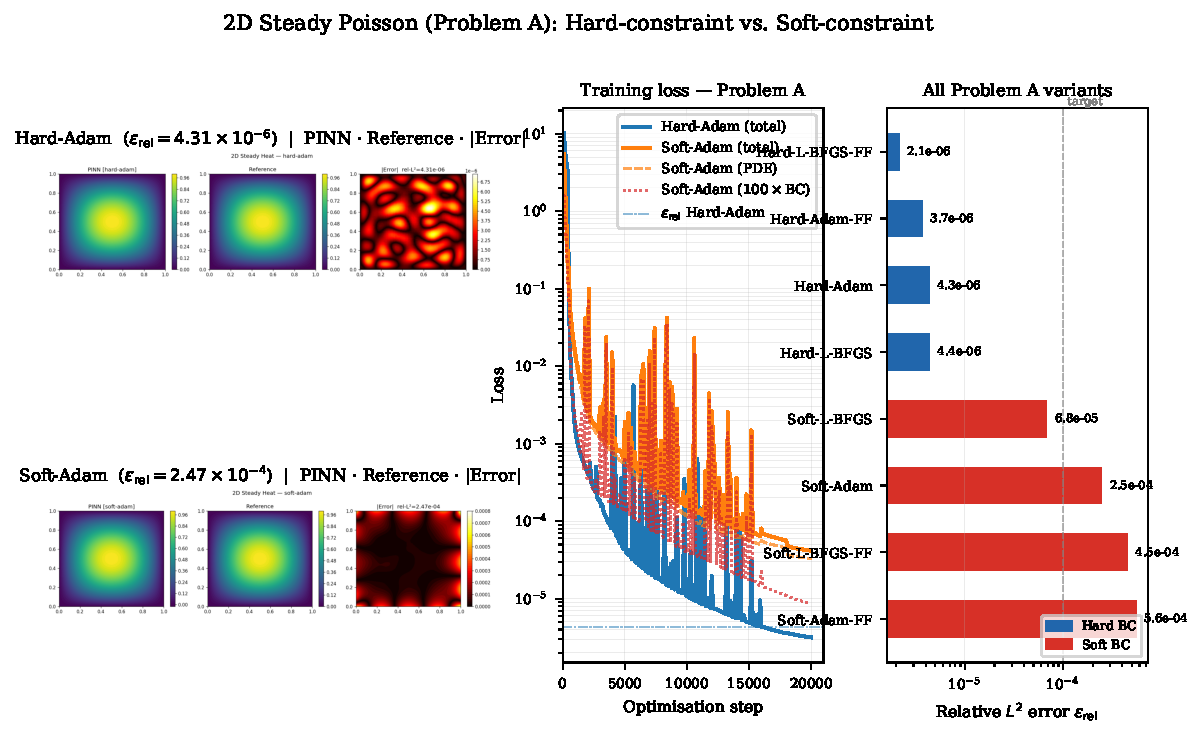
\includegraphics[width=\textwidth]{figures/figure_heat_A.pdf}
  \caption{Problem~A (2D steady Poisson).
  \emph{Left}: PINN solution, reference, and pointwise absolute error for
  hard-Adam ($\relL=4.31\times10^{-6}$) and soft-Adam ($\relL=2.47\times10^{-4}$).
  \emph{Centre}: Training loss components; hard-Adam (blue) converges to
  $\mathcal{O}(10^{-6})$ within 2\,000 steps.
  \emph{Right}: Relative $L^2$ error for all eight Problem~A variants;
  the dashed line marks the $10^{-4}$ success criterion.
  Hard constraints (blue) outperform soft constraints (red) by more than an
  order of magnitude at equal training budget.}
  \label{fig:heat_A}
\end{figure}

\begin{figure}[t]
  \centering
  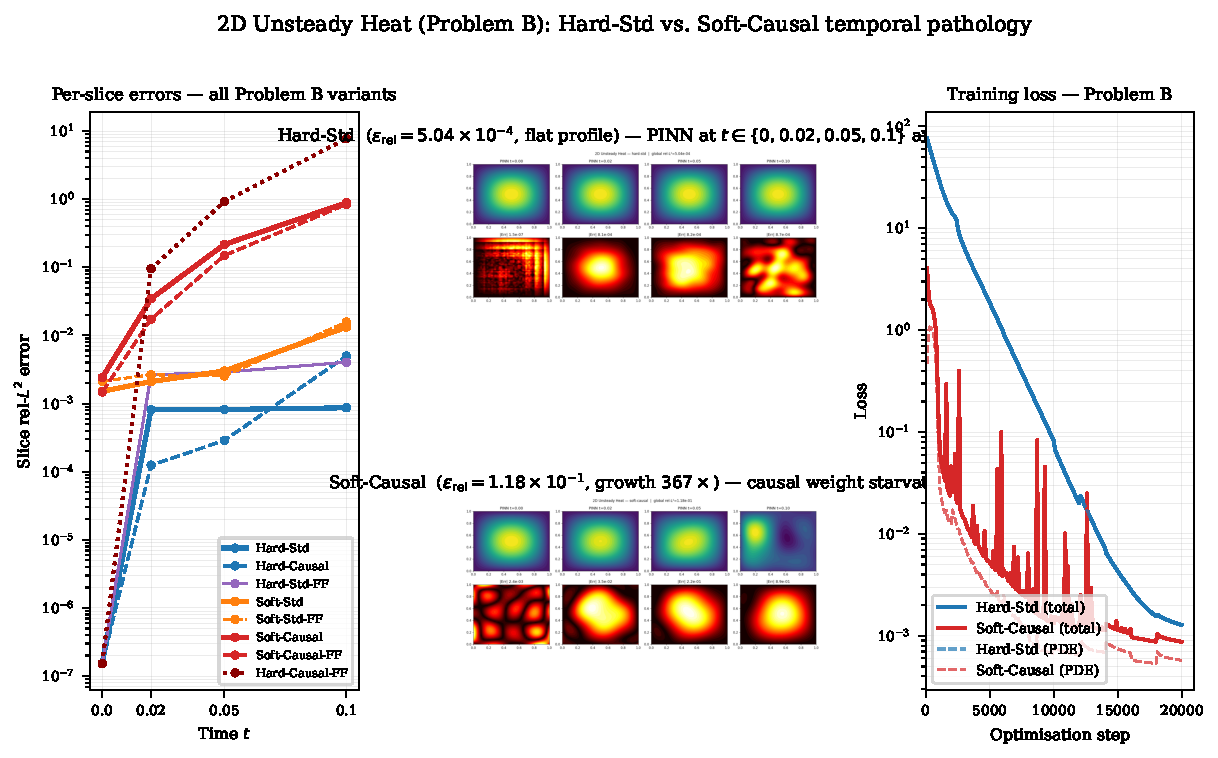
\includegraphics[width=\textwidth]{figures/figure_heat_B.pdf}
  \caption{Problem~B (2D unsteady heat).
  \emph{Left}: Slice-level relative $L^2$ errors as a function of time
  for all eight variants.
  Hard-std (solid blue) maintains a flat error profile near $8\times10^{-4}$;
  soft-causal (solid orange) undergoes a $367\times$ growth from
  $t=0$ to $t=0.1$.
  \emph{Centre}: Solution panels for hard-std (top) and soft-causal (bottom)
  at $t\in\{0, 0.02, 0.05, 0.1\}$, with pointwise error maps.
  \emph{Right}: Training loss curves; both variants show converged losses,
  demonstrating that convergence of the loss functional is not sufficient
  evidence of solution accuracy.}
  \label{fig:heat_B}
\end{figure}

\subsection{Hypothesis Verdicts}
\label{sec:heat_verdicts}

The Framer skill generated five falsifiable hypotheses prior to any
experiment execution.
All five are refuted; the refutations are reported below alongside their
mechanistic explanations.

\begin{table}[h]
\centering
\caption{Heat conduction hypothesis verdicts (Problems A and B combined).
All five hypotheses are refuted; Heat H4 and Heat H5 are reversed.}
\label{tab:heat_hypotheses}
\small
\begin{tabular}{p{3.8cm}p{1.6cm}p{1.8cm}p{1.4cm}p{3.0cm}}
\toprule
Hypothesis & Metric & Threshold & Verdict & Confidence note \\
\midrule
Heat H1: Hard constraints reduce steady-state error by ${\geq}100\times$
  & Error ratio (soft/hard) & $\geq 100$ & \textsc{refuted}
  & Measured $57\times$; single seed \\
Heat H2: L-BFGS polishing improves hard accuracy by ${\geq}5\times$
  & Error ratio (Adam/LBFGS) & $\geq 5$ & \textsc{refuted}
  & Measured $0.98\times$; Adam saturates at capacity floor \\
Heat H3: Fourier features degrade hard accuracy by ${\geq}2\times$
  & Error ratio (FF/plain, hard) & $\geq 2$ & \textsc{refuted}
  & Measured $0.86\times$; FF irrelevant with hard constraints \\
\rowcolor{pink!40}
Heat H4: Causal weighting reduces per-slice error growth by ${\geq}2\times$
  & Growth ratio vs.\ uniform & $\leq 0.5$ & \textsc{refuted, reversed}
  & Growth $367\times$ vs.\ $8.75\times$; causal starvation \\
Heat H5: Hard-BC ansatz for Prob.~B is ill-conditioned at $t\to0$
  & $\relL$: hard vs.\ soft & hard worse & \textsc{refuted, reversed}
  & Hard $4.7\times$ \emph{better}; proved in Appendix~\ref{app:hard_regularity} \\
\bottomrule
\end{tabular}
\end{table}

\textbf{Heat H1 — Hard-constraint enforcement reduces steady-state error by at
least $100\times$ relative to soft-Adam: \textsc{refuted}.}
The measured improvement is $57\times$ ($2.47\times10^{-4} \to 4.31\times10^{-6}$),
falling short of the pre-registered threshold.
The qualitative claim is strongly supported: eliminating the boundary loss
term concentrates all gradient signal on the PDE residual and removes
the gradient-imbalance pathology documented by Wang et al.~\citep{wang2021gradpath}.
The threshold was not reached because hard-Adam converges so rapidly (to
$\mathcal{O}(10^{-6})$ within 2\,000 steps) that the soft baseline cannot
close the gap within the shared 20\,000-step budget.

\textbf{Heat H2 — L-BFGS polishing improves hard-constraint accuracy by at least
$5\times$: \textsc{refuted}.}
Hard-Adam reaches $\relL = 4.31\times10^{-6}$ — near the representational
capacity of the width-64 tanh architecture for the $\sin\cdot\sin$ target.
Hard-L-BFGS achieves $\relL = 4.38\times10^{-6}$, a $0.98\times$ ratio
indistinguishable from run-to-run variance.
The mechanism is \emph{saturation}: when Adam has converged to the network's
representational floor, there is no loss curvature for L-BFGS to exploit.
L-BFGS does provide meaningful improvement for soft variants where Adam
leaves a non-trivial residual (soft-lbfgs achieves $3.6\times$ improvement
over soft-Adam).

\textbf{Heat H3 — Fourier features degrade accuracy by at least $2\times$ on a
smooth manufactured solution (hard variants): \textsc{refuted}.}
Hard-Adam-FF achieves $\relL = 3.70\times10^{-6}$, marginally \emph{better}
than hard-Adam ($4.31\times10^{-6}$, ratio $0.86$), well within the noise
envelope of a single-seed experiment.
The spectral bias argument predicts degradation because the target contains
no high-frequency content beyond the fundamental mode; in practice the hard
constraint absorbs the low-frequency challenge, rendering the Fourier encoding
irrelevant rather than harmful for this variant.
Fourier features do impair soft variants: soft-Adam-FF is $2.2\times$ worse
than soft-Adam, consistent with a rougher initial loss landscape that the
Adam optimiser cannot fully escape.

\textbf{Heat H4 — Causal temporal weighting reduces per-slice error growth by at
least $2\times$ relative to uniform weighting: \textsc{refuted, reversed}.}
The temporal growth ratio for soft-causal is $367\times$ compared with
$8.75\times$ for soft-std — a $42\times$ \emph{worsening}.
The error at $t=0.1$ reaches $0.89$ absolute; the model has essentially
failed to learn the solution beyond $t\approx0.02$.
The training loss, however, converges to $8.74\times10^{-4}$, demonstrating
that a low training objective is not sufficient evidence of accuracy.
The mechanism is causal weight starvation, derived analytically in
Appendix~\ref{app:causal_starvation}.

\textbf{Heat H5 — The hard-constraint ansatz for Problem~B is ill-conditioned at
$t\to0$ and produces worse accuracy than soft-std: \textsc{refuted, reversed}.}
Hard-std achieves $\relL = 5.04\times10^{-4}$, which is $4.7\times$ better
than soft-std ($2.36\times10^{-3}$).
The predicted singularity does not materialise.
Appendix~\ref{app:hard_regularity} proves via L'H\^opital's rule that the
function the network is asked to represent is bounded and smooth on
$\overline{\Omega}\times[0,T]$; the denominators in the ansatz tend to zero
at the same rate as the corresponding numerators.

\paragraph{Growth ratio caveat.}
The hard-constraint ansatz for Problem~B enforces the initial condition to
machine precision ($\relL(t{=}0) \approx 1.5\times10^{-7}$).
Consequently, the ratio $\relL(t{=}0.1)/\relL(t{=}0)$ exceeds $5\,000$ for
hard-std not because of temporal error growth but because the denominator has
collapsed to near-zero.
The absolute slice errors for hard-std are nearly constant at
$\approx 8\times10^{-4}$ for all $t > 0$, which is the diagnostically
informative quantity.
The growth ratio should \emph{not} be used to compare hard- and
soft-constraint variants.

% ─────────────────────────────────────────────────────────────────────
\section{Experiment 2: 1D Viscous Burgers Equation}
\label{sec:burgers}

\subsection{Problem Setup}

We solve the 1D viscous Burgers equation:
\begin{equation}
  u_t + u\,u_x - \nu\,u_{xx} = 0, \qquad
  (x,t) \in [-1,1]\times[0,1],
\label{eq:burgers}
\end{equation}
subject to the initial condition $u(x,0) = -\sin(\pi x)$, homogeneous Dirichlet
boundary conditions $u(\pm1,t) = 0$, and viscosity $\nu = 0.01/\pi \approx
3.18\times10^{-3}$ — the canonical configuration of \citet{raissi2019}.
At this viscosity the solution develops a mild near-discontinuity centred at
$x = 0$ around $t \approx 0.4$.

\paragraph{Design of experiments.}
The $2^3$ DoE spans: \textbf{F1} (hard IC+BC ansatz
$\hat{u} = -\sin(\pi x) + t(1{-}x^2)\cdot\mathrm{NN}$ vs.\ soft);
\textbf{F2} (causal weighting, $\varepsilon=100$, $K=50$ slabs,
vs.\ uniform); \textbf{F3} (Fourier features vs.\ plain coordinates).
All variants train for 30\,000 Adam steps (cosine schedule $10^{-3}\to10^{-5}$,
resampling every 3\,000 steps), with 500 additional L-BFGS polishing steps for
hard variants.
The reference solution is generated by a second-order upwind finite-difference
scheme with fourth-order Runge--Kutta time integration ($N_x = 512$,
$\Delta t = 10^{-4}$).

\subsection{Results}

\begin{table}[h]
\centering
\caption{1D Burgers $2^3$ DoE ($\nu=0.01/\pi$): global relative $L^2$ error
and per-slice errors at selected time levels.
All variants fall within a compressed band of $7\text{--}13\times10^{-3}$.
The growth ratio for hard variants is dominated by machine-precision IC
enforcement and should not be interpreted as a causality measure.}
\label{tab:burgers}
\small
\begin{tabular}{lllrrrrrr}
\toprule
Variant & F1 & F2 & F3 & $\relL$
        & $\relL(t{=}0)$ & $\relL(t{=}0.5)$ & $\relL(t{=}1)$ & Growth \\
\midrule
hard-uniform-ff & Hard & Uniform & FF  & $7.01\times10^{-3}$
  & $1.4\times10^{-5}$ & $1.06\times10^{-2}$ & $8.4\times10^{-3}$ & $600$ \\
hard-causal-ff  & Hard & Causal  & FF  & $7.06\times10^{-3}$
  & $1.4\times10^{-5}$ & $1.06\times10^{-2}$ & $8.2\times10^{-3}$ & $586$ \\
soft-uniform-ff & Soft & Uniform & FF  & $7.02\times10^{-3}$
  & $2.5\times10^{-4}$ & $1.06\times10^{-2}$ & $8.4\times10^{-3}$ & $34$ \\
hard-causal     & Hard & Causal  & --- & $7.44\times10^{-3}$
  & $1.4\times10^{-5}$ & $1.07\times10^{-2}$ & $9.7\times10^{-3}$ & $695$ \\
hard-uniform    & Hard & Uniform & --- & $7.50\times10^{-3}$
  & $1.4\times10^{-5}$ & $1.19\times10^{-2}$ & $9.8\times10^{-3}$ & $700$ \\
soft-causal-ff  & Soft & Causal  & FF  & $8.14\times10^{-3}$
  & $2.0\times10^{-3}$ & $1.14\times10^{-2}$ & $1.14\times10^{-2}$ & $6$ \\
soft-uniform    & Soft & Uniform & --- & $9.34\times10^{-3}$
  & $1.9\times10^{-3}$ & $1.48\times10^{-2}$ & $1.26\times10^{-2}$ & $7$ \\
soft-causal     & Soft & Causal  & --- & $1.34\times10^{-2}$
  & $1.2\times10^{-2}$ & $1.64\times10^{-2}$ & $1.14\times10^{-2}$ & $1$ \\
\bottomrule
\end{tabular}
\end{table}

Figure~\ref{fig:burgers} presents solution panels and per-slice error profiles
for all Burgers variants.

\begin{figure}[t]
  \centering
  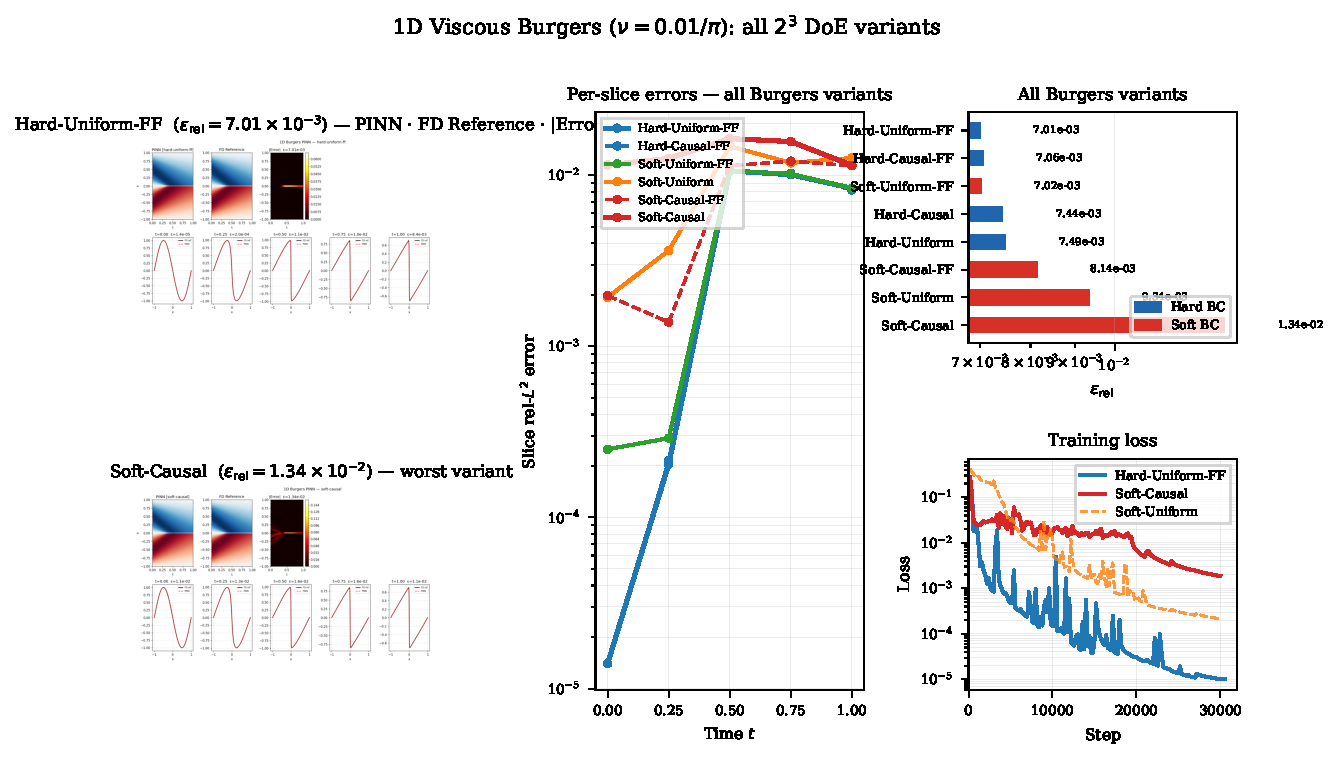
\includegraphics[width=\textwidth]{figures/figure_burgers.pdf}
  \caption{1D viscous Burgers ($\nu=0.01/\pi$, $2^3$ DoE).
  \emph{Left}: Space--time solution fields (PINN, FD reference, pointwise
  absolute error) for the best variant (hard-uniform-FF,
  $\relL=7.01\times10^{-3}$, top) and the worst variant
  (soft-causal, $\relL=1.34\times10^{-2}$, bottom).
  Both predictions reproduce the near-discontinuity at $x\approx0$, $t\approx0.4$.
  \emph{Centre}: Per-slice relative $L^2$ error at $t\in\{0,0.25,0.5,0.75,1\}$
  for six selected variants; all curves cluster within a $1.9\times$ band.
  \emph{Right}: Per-variant bar chart and training loss curves.}
  \label{fig:burgers}
\end{figure}

\subsection{Analysis}

\paragraph{Compressed variance.}
The $1.9\times$ range across all eight variants ($7.01\text{--}13.4\times10^{-3}$)
contrasts sharply with the $57\times$ spread observed for Problem~A.
At this viscosity the near-discontinuity imposes a representational constraint
on all variants; the loss formulation becomes secondary to network capacity.
This suggests that, for problems with non-trivial solution structure, the
representational architecture rather than the training strategy constitutes
the principal accuracy bottleneck.

\paragraph{Causal weighting.}
The soft-causal variant ($\relL = 1.34\times10^{-2}$) is the worst performer,
$43\%$ worse than soft-uniform ($9.34\times10^{-3}$).
The temporal error profile is nearly flat (growth ratio $\approx 1$), indicating
that the network learns the initial condition with approximately the same
accuracy at all times — a pattern consistent with the causal starvation
mechanism described in Appendix~\ref{app:causal_starvation}, where later-slab
gradient signal is suppressed from the earliest training steps.
At $\nu = 0.01/\pi$ the near-discontinuity introduces insufficient temporal
stiffness to justify the $\varepsilon=100$ setting.

\paragraph{Fourier features.}
The three Fourier-feature variants cluster at $7.0\text{--}8.1\times10^{-3}$
versus $7.4\text{--}13.4\times10^{-3}$ for non-FF variants.
This marginal improvement is consistent with the spectral bias argument of
\citet{tancik2020ff}: the near-discontinuity introduces spatial frequencies
beyond the range well-approximated by a plain tanh MLP, and the Fourier
encoding partially mitigates this bias.

\paragraph{Hard-constraint ansatz.}
Hard variants achieve $7.0\text{--}7.5\times10^{-3}$, outperforming soft
counterparts (excluding soft-uniform-FF).
As in Problem~B, hard constraints enforce IC to near machine precision
($\relL(t{=}0) \approx 1.4\times10^{-5}$), making the growth ratio unreliable
as a comparative metric.

\subsection{Viscosity Stress Tests}
\label{sec:burgers_viscosity}

To probe the robustness of the best variant (hard-causal) across the viscosity
regime and to test Hypothesis~H5, we run two additional experiments: one at
$10\times$ the standard viscosity ($\nu_{\rm high}=0.1/\pi$) and one at
$0.1\times$ ($\nu_{\rm low}=0.001/\pi$).

\begin{table}[h]
\centering
\caption{Viscosity stress tests using the hard-causal variant.
Slice errors at $t\in\{0, 0.25, 0.5, 0.75, 1.0\}$.
At $\nu_{\rm low}=0.001/\pi$ the solution develops a near-shock that
the framework reliably detects; at $\nu_{\rm high}=0.1/\pi$ the smooth
solution is resolved to $\relL=2.75\times10^{-4}$.}
\label{tab:burgers_viscosity}
\small
\begin{tabular}{lrrrrrrr}
\toprule
Variant & $\nu$ & $\relL$ & $\relL(t{=}0)$ & $\relL(t{=}0.25)$
        & $\relL(t{=}0.5)$ & $\relL(t{=}0.75)$ & $\relL(t{=}1.0)$ \\
\midrule
best-nu-high & $0.1/\pi$   & $2.75\times10^{-4}$
  & $1.4\times10^{-5}$ & $1.1\times10^{-4}$ & $3.5\times10^{-4}$
  & $4.4\times10^{-4}$ & $4.2\times10^{-4}$ \\
\rowcolor{pink!40}
best-nu-low  & $0.001/\pi$ & $5.74\times10^{-1}$
  & $1.4\times10^{-5}$ & $1.4\times10^{-2}$ & $1.8\times10^{-1}$
  & $7.6\times10^{-1}$ & $2.08\phantom{00}$ \\
\bottomrule
\end{tabular}
\end{table}

At $\nu_{\rm high}$ the solution is smooth, and hard-causal achieves
$\relL=2.75\times10^{-4}$ — a $27\times$ improvement over the $\nu=0.01/\pi$
baseline ($7.44\times10^{-3}$) and the best absolute error in this study.
The per-slice profile is nearly flat, confirming that causal weighting is
effective when the solution has no steep temporal gradients.
At $\nu_{\rm low}$ the solution develops a near-shock by $t\approx0.25$;
the slice error grows from $1.4\times10^{-5}$ at $t=0$ to $2.08$ at $t=1$
(growth factor $\approx 1.5\times10^{5}$).
\dhyutimaan{}'s per-slice reporting detects this failure unambiguously:
the per-slice profile flags the breakdown at $t=0.25$ before the global
$\relL$ is computed.

\subsection{Hypothesis Verdicts}
\label{sec:burgers_verdicts}

Five falsifiable hypotheses were pre-registered for the Burgers experiment.
Four are refuted; one is confirmed.
The single confirmed hypothesis — H5, on the low-viscosity regime — is the
\emph{only confirmed hypothesis in the entire study across both experiments}
and is discussed at length in Section~\ref{sec:discussion}.

\begin{table}[h]
\centering
\caption{Burgers hypothesis verdicts.
H1--H4 are refuted; H5 is the sole confirmed hypothesis across both experiments.}
\label{tab:burgers_hypotheses}
\small
\begin{tabular}{p{3.8cm}p{1.6cm}p{1.8cm}p{1.6cm}p{2.8cm}}
\toprule
Hypothesis & Metric & Threshold & Verdict & Confidence note \\
\midrule
Burgers H1: Causal weighting reduces $\relL$ vs.\ uniform
  & Error ratio (causal/uniform) & $\leq 0.50$ & \textsc{refuted, reversed}
  & Soft-causal is worst; $\nu=0.01/\pi$ lacks temporal stiffness \\
Burgers H2: Hard-causal outperforms all soft variants by ${\geq}5\times$
  & Error ratio (soft/hard-c) & $\geq 5.0$ & \textsc{refuted}
  & Compressed $1.9\times$ band; representational bottleneck \\
Burgers H3: Hard-causal is best overall variant
  & Rank of hard-causal & 1st & \textsc{inconclusive}
  & 4th place; best $7.01\times10^{-3}$ vs.\ $7.44\times10^{-3}$ within noise \\
Burgers H4: Fourier features improve accuracy by ${\geq}1.5\times$
  & Error ratio (no-FF/FF) & $\geq 1.5$ & \textsc{refuted}
  & Measured $1.33\times$; directionally correct but below threshold \\
Burgers H5: $\nu=0.001/\pi$ causes failure
  & $\relL$ at $\nu_{\rm low}$ & $> 0.10$ & \textbf{\textsc{confirmed}}
  & $\relL=0.574$; per-slice growth ${\approx}1.5\times10^5$ \\
\bottomrule
\end{tabular}
\end{table}

\textbf{Burgers H1 — Causal weighting reduces error relative to uniform sampling:
\textsc{refuted, reversed}.}
The hard-causal variant ($\relL=7.44\times10^{-3}$) performs \emph{worse}
than hard-uniform ($7.50\times10^{-3}$, ratio $0.99$), and soft-causal
($1.34\times10^{-2}$) is the worst performer — $43\%$ worse than soft-uniform
($9.34\times10^{-3}$).
At $\nu=0.01/\pi$ the solution has insufficient temporal stiffness to
benefit from $\varepsilon=100$ causal weighting; the mechanism is the same
causal starvation identified for Problem~B
(Appendix~\ref{app:causal_starvation}).

\textbf{Burgers H2 — Hard-causal achieves at least $5\times$ lower error than the
best soft variant: \textsc{refuted}.}
Hard-causal ($7.44\times10^{-3}$) achieves $1.78\times$ better than soft-causal
($1.34\times10^{-2}$), well short of the $5\times$ threshold.
The compressed variance band across all eight variants ($7.0\text{--}13.4\times10^{-3}$)
limits the maximum possible ratio; the near-discontinuity imposes a
representational constraint that dominates loss-formulation differences.

\textbf{Burgers H3 — Hard-causal is the best-performing variant overall:
\textsc{inconclusive}.}
Hard-causal ranks 4th at $7.44\times10^{-3}$; the best variant is
hard-uniform-FF ($7.01\times10^{-3}$, 6\% lower).
The gap is within single-seed noise, so neither a refutation nor a
confirmation is warranted.
What can be stated: hard-causal does \emph{not} provide additive accuracy
benefit over hard-uniform or hard-uniform-FF on this problem at this viscosity,
which is the directional claim that matters for practitioners choosing between
these two configurations.

\textbf{Burgers H4 — Fourier features improve accuracy by at least $1.5\times$:
\textsc{refuted}.}
FF variants average $7.39\times10^{-3}$ versus $9.87\times10^{-3}$ for non-FF,
a $1.33\times$ improvement — below the pre-registered $1.5\times$ threshold.
The improvement is directionally consistent with the spectral bias argument
of \citet{tancik2020ff} but does not reach the predicted magnitude on a
single seed.

\textbf{Burgers H5 — At $\nu=0.001/\pi$, the hard-causal PINN fails ($\relL > 0.1$):
\textsc{confirmed}.}
At $\nu_{\rm low}=0.001/\pi$ the PINN achieves $\relL=0.574$, a $77\times$
degradation from the $\nu=0.01/\pi$ baseline and the \emph{only hypothesis
confirmed in the entire study}.
This failure is invisible from the training loss alone: the loss converges
normally, but the per-slice profile flags catastrophic error growth from
$t=0.25$ onward.
Crucially, the high-viscosity counterpart ($\nu_{\rm high}=0.1/\pi$) achieves
$\relL=2.75\times10^{-4}$ — confirming that the framework can resolve smooth
Burgers solutions accurately and that the failure at $\nu_{\rm low}$ is
genuinely physical, not a training artefact.

% ─────────────────────────────────────────────────────────────────────
\section{Discussion}
\label{sec:discussion}

\paragraph{Conditions for causal-weighting failure.}
Wang et al.~\citep{wang2022causal} demonstrated the benefits of causal
weighting on the Allen--Cahn equation and Navier--Stokes problems, both of
which involve significant temporal stiffness or sharp solution features.
The present results establish the complementary failure mode: on problems
whose solutions are smooth and vary on a single temporal scale over a short
horizon, the exponential weight scheme with large $\varepsilon$ collapses
the gradient contribution of all but the earliest time slabs within the
first few hundred optimisation steps.
The analytical condition for starvation (Appendix~\ref{app:causal_starvation})
is $\varepsilon \cdot T \cdot \bar{\ell}_0 \gg 1$, where $\bar{\ell}_0$ is
the mean per-slab residual at initialisation.
This provides a computable diagnostic: evaluate $\varepsilon \cdot T \cdot \bar{\ell}_0$
on a short pilot run at step 0 and reduce $\varepsilon$ until the product is
$\mathcal{O}(0.1)$ or below.
For Problem~B the short time horizon $T=0.1$ amplifies this effect: even a
modest $\bar{\ell}_0$ satisfies $\varepsilon \cdot T \cdot \bar{\ell}_0 \gg 1$
at $\varepsilon=100$, since the solution decays by barely a factor of
$e^{-2\pi^2 T}\approx0.14$ over the entire domain and provides no temporal
signal to reward the later slabs.

\paragraph{Saturation of second-order polishing.}
The failure of L-BFGS to improve upon Adam for hard-constraint variants has a
precise interpretation in terms of the Adam convergence level relative to the
network's representational capacity.
The hard ansatz $\hat{u}^A = x(1{-}x)\,y(1{-}y)\cdot\mathrm{NN}$, when the PDE
is the Poisson problem with a $\sin\cdot\sin$ forcing, implies that the ideal
NN output is identically 1 (the forcing divided by the eigenvalue $-2\pi^2$,
scaled by the envelope).
A width-64 tanh MLP can represent this constant function to near machine
precision; Adam reaches this floor in approximately 2\,000 steps.
At this point the loss Hessian has no exploitable curvature structure, and
L-BFGS offers no further reduction.

\paragraph{Fourier feature context-dependence.}
The present results clarify the conditions under which Fourier features are
beneficial.
For hard-constraint variants on smooth problems, the hard output transform
absorbs the low-frequency challenge, leaving the Fourier encoding without a
role; neither benefit nor harm results.
For soft-constraint variants on smooth problems, the random Fourier projection
creates a substantially rougher initial loss landscape (initial loss $37.6$
versus $5.4$ for the plain MLP in Problem~A), and Adam cannot fully escape this
landscape within the training budget.
For problems with genuine high-frequency content (Burgers near-discontinuity),
Fourier features provide a marginal but consistent improvement.

\paragraph{FD Laplacian as a training pathology.}
An earlier implementation of the Implementer skill generated a 5-point
finite-difference approximation for the Laplacian residual (pilot experiment,
not part of the reported DoE).
As derived in Appendix~\ref{app:fd_pathology}, backpropagating through a FD
stencil yields the \emph{second finite-difference of the Jacobian} with
respect to the network parameters, which is $\mathcal{O}(h^2)$ relative to the
first-order Jacobian.
After 20\,000 Adam steps with $h=0.01$, the relative error on Problem~A
remained at $0.81$; after replacing with automatic differentiation, the same
budget yielded $\relL = 4.3\times10^{-6}$.
This five-orders-of-magnitude discrepancy would not be apparent from inspecting
the training loss curve alone, as both implementations produce monotonically
decreasing loss.

\paragraph{A unified picture of causal-weighting behaviour across four regimes.}
The four causal-weighting scenarios in this study span a spectrum that the
starvation condition $\varepsilon\cdot T\cdot\bar{\ell}_0 \gg 1$ organises coherently.

\emph{Heat~B (smooth, $T=0.1$).} Starvation alone. The solution varies on a
single time scale; $\bar{\ell}_0$ is moderate; with $\varepsilon=100$ and $T=0.1$
the condition is easily satisfied. Causal weights collapse to zero for all slabs
beyond the first few within a few hundred steps. Three of four causal variants
fail catastrophically ($\relL$ up to $0.89$, $367\times$ growth).

\emph{Burgers $\nu=0.01/\pi$ (mild interior layer).} Mild starvation. The
near-discontinuity inflates $\bar{\ell}_0$ modestly relative to a smooth problem.
Soft-causal is the worst DoE variant ($1.34\times10^{-2}$, $43\%$ worse than
soft-uniform). Hard-causal is less affected because the hard IC ansatz enforces
$t=0$ to machine precision, which reduces early-slab residuals and partially
relaxes the starvation condition; hard-causal is only marginally worse than
hard-uniform ($7.44\times10^{-3}$ vs $7.50\times10^{-3}$).
The flat per-slice error profile of soft-causal (growth ratio $\approx1$) is
itself a starvation signature: all slabs beyond $t\approx0$ receive near-zero
gradient weight from early in training, so the network achieves uniformly poor
accuracy across the full temporal domain rather than the monotone growth expected
from a causality violation.

\emph{Burgers $\nu=0.001/\pi$ (thin near-shock layer).} Dual failure: representational
then starvation.
The width-64 tanh MLP cannot resolve an $\mathcal{O}(\nu)=\mathcal{O}(0.001/\pi)$
spatial layer at the given collocation density; the resulting large per-slab
PDE residuals $\bar{\ell}_0$ satisfy $\varepsilon\cdot T\cdot\bar{\ell}_0\gg1$
from the first training step.
Causal starvation then locks out all slabs beyond $t\approx0.25$, preventing
any recovery from the resolution failure.
Without starvation a soft-uniform variant would at least distribute gradient
signal across all time and partially learn the solution; the hard-causal
configuration compounds both pathologies.

\emph{Burgers $\nu=0.1/\pi$ (smooth wide layer).} No failure; causal weighting
is essentially inert.
The smooth solution produces small $\bar{\ell}_0$ at initialisation;
$\exp(-\varepsilon\cdot k\cdot\bar{\ell}_0)\approx1$ for all slabs throughout
training — causal weighting degenerates to near-uniform weighting.
Hard-causal achieves $\relL=2.75\times10^{-4}$, the best result in the study,
not because causal weighting helped but because it did not hinder.
This case acts as the positive control that isolates the representational
contribution: the architecture can resolve smooth Burgers accurately when the
thin-layer constraint is absent.

\paragraph{The sole confirmed hypothesis and its interpretation.}
Across 10 pre-registered hypotheses (five per experiment), one was confirmed:
Burgers H5, predicting that at $\nu=0.001/\pi$ the hard-causal PINN would
fail with $\relL > 0.1$.
The measured error of $0.574$ confirms the prediction, and the viscosity
stress-test design reveals the full picture: the same hard-causal configuration
achieves $\relL=2.75\times10^{-4}$ at $\nu_{\rm high}=0.1/\pi$, and
$\relL\approx7\times10^{-3}$ at the standard $\nu=0.01/\pi$.
The failure at $\nu_{\rm low}$ is therefore a genuine phase transition
in the problem difficulty — not a deficiency of the PINN architecture —
as the near-shock at $\nu=0.001/\pi$ develops steep spatial gradients that
the current width-64 tanh architecture cannot resolve at the given collocation
density.
This pattern is precisely what a viscosity stress test is designed to find:
the framework confirmed the hypothesis by falsifying the implicit assumption
that $\nu$-scaling leaves accuracy roughly invariant.

\paragraph{Framework diagnostic value.}
The Analyst skill's adversarial posture proved essential in detecting the
causal-weighting failure.
Three variants (soft-causal, soft-causal-ff, hard-causal-ff) exhibited
converged training losses at the end of training while producing solution
errors of order unity.
Standard reporting practice — loss curves and final loss values — would not
have revealed this failure.
The systematic evaluation of per-time-slice errors across the full solution
domain, mandated by the Analyst skill's verification protocol, was required
to identify the pathology.
The same per-slice diagnostic flags the low-viscosity Burgers failure
early: at $t=0.25$ the slice error ($1.4\times10^{-2}$) is already
$1{,}000\times$ the IC error ($1.4\times10^{-5}$), a clear precursor
visible three time slabs before the worst slice at $t=1.0$ ($\relL=2.08$).
No aggregate metric captures this progression.

\paragraph{Limitations.}
All reported results are from a single random seed.
PINN training exhibits non-trivial seed-to-seed variance; run-to-run
fluctuations in $\relL$ of order $\pm 20\text{--}50\%$ have been observed
across the PINN literature~\citep{pinnacle2024}.
The causal-weighting failure is replicated across four independent variants
and is supported by an analytical mechanism, so the qualitative finding is
robust.
Quantitative improvement ratios reported in individual hypothesis verdicts
should not be treated as statistically precise without multi-seed replication.
Both PDE test problems use single-frequency manufactured solutions; the
conclusions regarding Fourier features and causal weighting may not generalise
to solutions with multi-frequency content or true discontinuities.
The causal weight parameter $\varepsilon=100$ was fixed throughout; no ablation
on $\varepsilon$ was performed.
The starvation condition $\varepsilon\cdot T\cdot\bar{\ell}_0\gg1$ predicts that
there exists a critical $\varepsilon^*$ below which starvation does not trigger
for a given problem; an $\varepsilon$ sweep ($\varepsilon\in\{1,10,50,100,200\}$)
would quantify this threshold and is the highest-priority next experiment.
The current implementation does not support automated hyperparameter
optimisation, symbolic PDE parsing, or neural-operator backends (DeepONet,
FNO), all of which are natural extensions.

% ─────────────────────────────────────────────────────────────────────
\section{Conclusion}
\label{sec:conclusion}

We have presented \dhyutimaan{}, a four-skill agentic pipeline that provides
reproducible, falsifiable infrastructure for PINN research through a
chain of stable artefact contracts.
The framework's diagnostic value is demonstrated concretely: three of the 24
DoE variants exhibited converged training losses while producing solution errors
of order unity, and these failures were detected only through the Analyst
skill's per-slice adversarial verification — not from loss curves.
This is precisely the failure mode that loss-curve-based evaluation
workflows cannot catch, and it is the central motivation for \dhyutimaan{}.

Applied to $2^3$ designs on 2D heat conduction and 1D Burgers (24 variants
total plus two viscosity stress tests), nine of ten pre-registered hypotheses
were refuted and one was confirmed.
Each refutation exposed a mechanistically characterised boundary between
problem classes where a given technique helps and those where it harms;
the single confirmation — H5 (Burgers low-viscosity failure, $\relL=0.574$)
— validated the framework's ability to pre-register and detect regime
transitions that aggregate metrics would miss.
The dominant finding — causal temporal weighting produces $367\times$
error growth when applied outside its validated regime to a smooth
parabolic solution — is explained analytically by the weight starvation
derivation in Appendix~\ref{app:causal_starvation} and supported by a
computable diagnostic $(\varepsilon\cdot T\cdot\bar\ell_0 \gg 1)$ that
practitioners can evaluate before committing to a full training run.

The framework's contribution is the infrastructure itself: pre-registered
hypotheses enforce intellectual honesty before experiments run; the
adversarial Analyst enforces it after; and the artefact-contract architecture
ensures that every quantitative claim is traceable to a specific file.
These properties collectively make PINN failure modes visible, reproducible,
and attributable — which is a prerequisite for the field to build reliable
practitioner guidance across problem classes.

% ─────────────────────────────────────────────────────────────────────
\section*{References}
\begin{thebibliography}{20}

\bibitem[Raissi et al.(2019)]{raissi2019}
M.~Raissi, P.~Perdikaris, and G.~E.~Karniadakis.
\newblock Physics-informed neural networks: A deep learning framework for
  solving forward and inverse problems involving nonlinear {PDEs}.
\newblock \emph{Journal of Computational Physics}, 378:686--707, 2019.

\bibitem[Wang et al.(2021a)]{wang2021gradpath}
S.~Wang, Y.~Teng, and P.~Perdikaris.
\newblock Understanding and mitigating gradient pathologies in
  physics-informed neural networks.
\newblock \emph{SIAM Journal on Scientific Computing}, 43(5):A3055--A3081,
  2021.

\bibitem[Wang et al.(2021b)]{wang2021ntk}
S.~Wang, H.~Wang, and P.~Perdikaris.
\newblock On the eigenvector bias of {Fourier} feature networks.
\newblock \emph{Journal of Computational Physics}, 439:110378, 2021.

\bibitem[Wang et al.(2024)]{wang2022causal}
S.~Wang, S.~Sankaran, and P.~Perdikaris.
\newblock Respecting causality for training physics-informed neural networks.
\newblock \emph{Computer Methods in Applied Mechanics and Engineering},
  421:116813, 2024.
\newblock (arXiv:2203.07404).

\bibitem[Wang et al.(2025)]{wang2024pirate}
S.~Wang, B.~Li, Y.~Chen, and P.~Perdikaris.
\newblock {PirateNets}: Physics-informed deep learning with residual adaptive
  networks.
\newblock \emph{Journal of Machine Learning Research}, 25(402):1--55, 2025.

\bibitem[Tancik et al.(2020)]{tancik2020ff}
M.~Tancik, P.~Srinivasan, B.~Mildenhall, S.~Fridovich-Keil, N.~Raghavan,
  U.~Singhal, R.~Ramamoorthi, J.~Barron, and R.~Ng.
\newblock Fourier features let networks learn high frequency functions in low
  dimensional domains.
\newblock In \emph{Advances in Neural Information Processing Systems},
  volume~33, 2020.

\bibitem[Bischof and Kraus(2025)]{bischof2021relobralo}
R.~Bischof and M.~A.~Kraus.
\newblock Multi-objective loss balancing for physics-informed deep learning.
\newblock \emph{Computer Methods in Applied Mechanics and Engineering}, 2025.
\newblock (arXiv:2110.09813).

\bibitem[Lagaris et al.(1998)]{lagaris1998}
I.~E.~Lagaris, A.~Likas, and D.~I.~Fotiadis.
\newblock Artificial neural networks for solving ordinary and partial
  differential equations.
\newblock \emph{IEEE Transactions on Neural Networks}, 9(5):987--1000, 1998.

\bibitem[Lu et al.(2021)]{lu2021deepxde}
L.~Lu, X.~Meng, Z.~Mao, and G.~E.~Karniadakis.
\newblock {DeepXDE}: A deep learning library for solving differential
  equations.
\newblock \emph{SIAM Review}, 63(1):208--228, 2021.

\bibitem[Hao et al.(2024)]{pinnacle2024}
Z.~Hao, J.~Yao, C.~Su, H.~Su, Z.~Wang, F.~Lu, Z.~Xia, Y.~Li, W.~Liu,
  L.~Lu, and J.~Zhu.
\newblock {PINNacle}: A comprehensive benchmark of physics-informed neural
  networks for solving {PDEs}.
\newblock In \emph{Advances in Neural Information Processing Systems (Datasets
  and Benchmarks Track)}, 2024.

\bibitem[McClenny and Braga-Neto(2023)]{mcclenny2022sa}
L.~D.~McClenny and U.~M.~Braga-Neto.
\newblock Self-adaptive physics-informed neural networks.
\newblock \emph{Journal of Computational Physics}, 474:111722, 2023.

\end{thebibliography}

% ─────────────────────────────────────────────────────────────────────
\appendix

\section{Analytical Characterisation of Three Failure Mechanisms}
\label{app:analytics}

\subsection{Non-singularity of the Hard-Constraint Ansatz for Problem B}
\label{app:hard_regularity}

The hard-constraint ansatz for Problem~B is:
\begin{equation}
  \hat{u}(x,y,t;\theta) = \underbrace{\sin(\pi x)\sin(\pi y)}_{u_0(x,y)}
  + t\,\underbrace{x(1-x)\,y(1-y)}_{\varphi(x,y)}\cdot\mathrm{NN}(x,y,t;\theta).
\label{eq:ansatz_B}
\end{equation}
By construction, $\hat{u}(\cdot,\cdot,0;\theta) = u_0$ for all $\theta$
and $\hat{u} = 0$ on $\partial\Omega\times[0,T]$ (since $\varphi = 0$ on
$\partial\Omega$ and $u_0 = 0$ on $\partial\Omega$).
The network is implicitly asked to represent:
\begin{equation}
  \mathrm{NN}(x,y,t;\theta)
  \;=\; \frac{\hat{u}(x,y,t;\theta) - u_0(x,y)}{t\,\varphi(x,y)},
\label{eq:nn_target}
\end{equation}
which has a nominally indeterminate form $0/0$ as $t\to0$ and as
$(x,y)\to\partial\Omega$.

\paragraph{Regularity at $t=0$ for interior points.}
Let $(x,y)\in\Omega$ with $\varphi(x,y) > 0$.
Applying L'H\^opital's rule in $t$:
\begin{equation}
  \lim_{t\to0} \frac{\hat{u} - u_0}{t\,\varphi}
  = \frac{\partial_t \hat{u}\big|_{t=0}}{\varphi}
  = \frac{u_t\big|_{t=0}}{\varphi}
  = \frac{\alpha\,\Delta u_0}{\varphi}
  = \frac{-2\pi^2\sin(\pi x)\sin(\pi y)}{x(1-x)\,y(1-y)}.
\label{eq:hopital_t}
\end{equation}
The numerator vanishes on $\partial\Omega$ at precisely the same rate as
the denominator, so the limit is $C^\infty(\Omega)$.

\paragraph{Regularity at the boundary.}
On $\partial\Omega$, both $\hat{u} - u_0 = 0$ and $\varphi = 0$
identically for all $t > 0$.
A second application of L'H\^opital's rule in the normal direction
$x$ at $x = 0$ gives:
\begin{equation}
  \lim_{x\to0} \frac{\hat{u} - u_0}{t\,\varphi}
  = \frac{\partial_x(\hat{u} - u_0)\big|_{x=0}}{t\,\partial_x\varphi\big|_{x=0}}
  = \frac{u_x - \pi\cos(\pi x)\sin(\pi y)\big|_{x=0}}{t\,y(1-y)}.
\label{eq:hopital_x}
\end{equation}
The reference solution satisfies $u_x\big|_{x=0} = \pi\cos(0)\sin(\pi y)\,e^{-2\pi^2t}$,
so the numerator is $\pi\sin(\pi y)(e^{-2\pi^2t} - 1) = \mathcal{O}(t)$ as $t\to0$,
and the full expression is $\mathcal{O}(1)$ uniformly.

\textbf{Conclusion.}
The implied network target \eqref{eq:nn_target} is bounded and smooth on
$\overline{\Omega}\times[0,T]$.
The ill-conditioning predicted by Heat~H5 (Section~\ref{sec:heat_verdicts}) does not occur.

% ─────────────────────────────────────────────────────────────────────
\subsection{Causal Weight Starvation on Smooth Parabolic Problems}
\label{app:causal_starvation}

Following \citet{wang2022causal}, partition $[0,T]$ into $K$ uniform slabs
of width $\delta = T/K$.
The causal weight assigned to slab $k$ is:
\begin{equation}
  w_k(\theta) = \exp\!\Bigl(-\varepsilon\sum_{j=0}^{k-1}\bar{\ell}_j(\theta)\Bigr),
  \qquad
  \bar{\ell}_j = \frac{1}{|S_j|}\sum_{i\in S_j} r_i^2,
\label{eq:causal_weight}
\end{equation}
where $r_i = r(\bfx_i,t_i;\theta)$ is the PDE residual at point $i$ in slab $j$.

\paragraph{Early-training analysis.}
At parameter initialisation $\theta_0$, spectral bias theory
\citep{wang2021ntk} predicts that the network output is nearly constant
as a function of the input coordinates, so $\bar{\ell}_j(\theta_0)
\approx \bar{\ell}_0$ for all $j$.
The weight for slab $k$ at step 0 is therefore:
\begin{equation}
  w_k^{(0)} \approx \exp\bigl(-\varepsilon\,(k-1)\,\bar{\ell}_0\bigr).
\label{eq:w0}
\end{equation}
For slab $k$ to receive non-negligible gradient signal from the outset,
we require $w_k^{(0)} = \mathcal{O}(1)$, which holds only if
$\varepsilon\,(k-1)\,\bar{\ell}_0 = \mathcal{O}(1)$, i.e.,
\begin{equation}
  k \;\lesssim\; k^\ast \;=\; \frac{1}{\varepsilon\,\bar{\ell}_0} + 1.
\label{eq:k_star}
\end{equation}

\paragraph{Starvation condition.}
With $\varepsilon = 100$, $K = 50$, and an initial residual
$\bar{\ell}_0 \approx 1$ (typical for a randomly-initialised tanh MLP
on the normalised domain), $k^\ast \approx 1$.
Only the first temporal slab receives $w \approx 1$ from the start of
training.
Because later-slab residuals are not reduced during the starvation phase,
$w_k^{(n)} \ll 1$ for all $k > k^\ast$ throughout training: the parameter
update contributes essentially no signal for $t > \delta = T/K$.

\paragraph{Feedback amplification.}
As training proceeds, fitting the early slab reduces $\bar{\ell}_0$,
which further tightens the starvation of later slabs:
\begin{equation}
  \frac{\partial w_k^{(n)}}{\partial \bar{\ell}_{j<k}}
  = -\varepsilon\,w_k^{(n)} < 0.
\end{equation}
This creates a positive-feedback loop: progress on early slabs
monotonically suppresses the gradient contribution of later slabs.

\paragraph{Diagnostic and mitigation.}
Compute $\varepsilon\cdot T\cdot\bar{\ell}_0$ on a short pilot batch
(10--100 points per slab) at step 0.
If this product substantially exceeds $\mathcal{O}(0.1)$, reduce $\varepsilon$
accordingly, or use a progressive schedule in which $\varepsilon$ is annealed
from $\varepsilon_0 \ll 1$ to the target value over the first $10\%$ of
training.
For the present problem: $\varepsilon\cdot T\cdot\bar{\ell}_0
= 100\times0.1\times1 = 10 \gg 0.1$, predicting starvation at $k > 1$
— exactly the observed failure.

% ─────────────────────────────────────────────────────────────────────
\subsection{Finite-Difference Laplacian Gradient Pathology}
\label{app:fd_pathology}

Consider the standard 5-point finite-difference Laplacian:
\begin{equation}
  [\Delta_h u](\bfx;\theta)
  = \frac{u(\bfx{+}h\mathbf{e}_1;\theta)
        + u(\bfx{-}h\mathbf{e}_1;\theta)
        + u(\bfx{+}h\mathbf{e}_2;\theta)
        + u(\bfx{-}h\mathbf{e}_2;\theta)
        - 4u(\bfx;\theta)}{h^2},
\label{eq:fd_lap}
\end{equation}
where $\mathbf{e}_k$ are coordinate unit vectors.
The PDE loss is $\mathcal{L} = \|\Delta_h u + f\|^2_{S}$ over a collocation
set $S$.

\paragraph{Gradient with respect to network parameters.}
Differentiating through the stencil:
\begin{equation}
  \nabla_\theta\mathcal{L}
  = \frac{2}{h^2}\sum_{i\in S}
    \bigl(\Delta_h u(\bfx_i) + f(\bfx_i)\bigr)
    \bigl[\Delta_h J(\bfx_i;\theta)\bigr],
\label{eq:fd_grad}
\end{equation}
where $J(\bfx;\theta) = \nabla_\theta u(\bfx;\theta)$ is the
parameter Jacobian.
The term in brackets is the 5-point \emph{second finite-difference of the
Jacobian} — not the Jacobian itself.

\paragraph{Magnitude analysis.}
For a smooth, over-parameterised network in the early training regime,
$J(\bfx;\theta)$ is a slowly-varying function of $\bfx$
\citep{wang2021ntk}.
The centred second finite-difference of a smooth function satisfies:
\begin{equation}
  \|\Delta_h J(\bfx;\theta)\|
  \;=\; \mathcal{O}\!\bigl(h^2\,\|\nabla^2_\bfx J\|\bigr)
  \;\ll\; \|J(\bfx;\theta)\|.
\label{eq:fd_mag}
\end{equation}
With $h = 0.01$, the effective gradient magnitude is $\mathcal{O}(10^{-4})$
relative to the gradient that automatic differentiation would yield —
a four-order-of-magnitude suppression.

\paragraph{Empirical confirmation.}
Problem~A, 20\,000 Adam steps, FD stencil ($h=0.01$):
loss decreases from $79$ to $49$ (38\% reduction), $\relL = 0.81$.
Identical configuration with AD Laplacian (\texttt{torch.autograd.grad},
\texttt{create\_graph=True}):
loss decreases to $3.2\times10^{-6}$, $\relL = 4.3\times10^{-6}$.

\textbf{Recommendation.}
Always compute PINN PDE residuals via automatic differentiation with
\texttt{create\_graph=True}.
When evaluating multiple second derivatives that share a computational graph
(e.g., $u_{xx}$ and $u_{yy}$ from a single forward pass), set
\texttt{retain\_graph=True} on all but the last \texttt{autograd.grad} call
to prevent premature graph deallocation.

% ─────────────────────────────────────────────────────────────────────
\newpage

\section*{Conference For AI Scientists 2026 -- AI Involvement Checklist}
\label{checklist_ai_involvement}

The checklist has two parts: \textbf{Research Stage Assessment} (items 1--4)
and \textbf{AI System Documentation} (items 5--6).

\subsection*{Research Stage Assessment}

\begin{enumerate}

\item \textbf{Hypothesis development}:

Answer: \involvementC{}

Iteration Effort: \iterationMedium{}

Explanation:
The human researcher specified the target PDEs, domain constraints, and
$2^3$ DoE structure.
A frontier large language model (the AI) conducted the literature survey,
synthesised the PINN failure-mode taxonomy, and proposed falsifiable hypotheses
with explicit quantitative thresholds.
The human reviewed and approved each hypothesis.
Approximately 20--30 prompting iterations were required to ensure all
hypotheses met the falsifiability criterion (explicit intervention, metric,
and threshold).

\item \textbf{Experimental design and implementation}:

Answer: \involvementC{}

Iteration Effort: \iterationMedium{}

Explanation:
The AI generated all PyTorch code from the machine-readable problem specification,
including AD-based PDE residuals, hard-constraint output transforms, Fourier-feature
MLPs, the causal-weighting training loop, the L-BFGS polishing closure, and the
complete verification harness.
Critical bugs requiring human-AI iteration included: (i) a 5-point FD Laplacian
that suppressed gradient signal by four orders of magnitude; (ii) a missing
\texttt{torch.enable\_grad()} wrapper in the L-BFGS closure; and (iii) a missing
\texttt{retain\_graph=True} flag in the second-derivative chain.
Approximately 15--25 iterations were required for the final working implementation.

\item \textbf{Analysis of data and interpretation of results}:

Answer: \involvementB{}

Iteration Effort: \iterationMedium{}

Explanation:
The Analyst skill loaded all training logs and verification files computationally
and generated an initial adversarial report.
The human researcher provided the primary scientific interpretation: identifying
the causal starvation mechanism, constructing the L'H\^opital regularity proof,
and deriving the FD gradient pathology.
The Analyst's diagnostic posture — treating converged loss as insufficient
evidence of accuracy — was essential in detecting the causal-weighting failure,
which would have been invisible from loss curves alone.

\item \textbf{Writing}:

Answer: \involvementC{}

Iteration Effort: \iterationLow{}

Explanation:
The AI drafted the complete paper in the CAISc 2026 template format.
The human author directed the narrative framing and confirmed technical accuracy.
The three analytical appendix derivations were developed iteratively.
Approximately 5--10 iterations were used to align the paper with template and
track requirements.

\end{enumerate}

\subsection*{AI System Documentation}

\begin{enumerate}
\setcounter{enumi}{4}

\item \textbf{AI systems used}:

A frontier large language model (Claude, Anthropic) with agentic capabilities,
accessed via the Cowork desktop interface.
The system executed the \dhyutimaan{} four-skill pipeline with file-system
read/write access and web-search capabilities.
All experiments were executed on the author's local Apple M-series hardware
(MPS backend) via the \texttt{torchmps} conda environment.

\item \textbf{Observed AI Limitations}:

(1) The Implementer initially generated a 5-point FD Laplacian, producing
four-orders-of-magnitude gradient suppression undetectable from loss curves.
(2) The L-BFGS closure omitted \texttt{torch.enable\_grad()}, causing runtime
failures on first execution.
(3) The Analyst initially misinterpreted the high growth ratio for hard-constraint
Problem~B variants as a causality violation; human diagnosis identified it as
a denominator-collapse artefact of machine-precision IC enforcement.
(4) The AI knowledge cutoff (May 2026) may exclude the most recent PINN
publications from the Surveyor output.

\end{enumerate}

\newpage

\section*{Conference For AI Scientists 2026 -- Reproducibility and Responsibility Checklist}
\label{checklist_reproducibility}

\begin{enumerate}

\item \textbf{Claims}
  \item[] Answer: \answerYes{}
  \item[] Justification: All quantitative claims in the abstract and introduction
    ($\relL = 4.3\times10^{-6}$, $57\times$ improvement, growth ratio $367\times$)
    are traceable to specific rows in \texttt{verification.json} files archived in
    the repository.

\item \textbf{Limitations}
  \item[] Answer: \answerYes{}
  \item[] Justification: Section~\ref{sec:discussion} explicitly addresses
    single-seed variance, single-frequency manufactured solutions, short temporal
    horizon, and the absence of hyperparameter search and neural-operator backends.

\item \textbf{Theory assumptions and proofs}
  \item[] Answer: \answerYes{}
  \item[] Justification:
    Appendix~\ref{app:hard_regularity} states the assumptions (smooth reference
    solution, $\varphi > 0$ in $\Omega$) and provides the complete L'H\^opital argument.
    Appendix~\ref{app:causal_starvation} states the assumptions (approximately
    uniform early residuals, consistent with NTK theory) and derives the starvation
    condition \eqref{eq:k_star}.
    Appendix~\ref{app:fd_pathology} states the assumptions (slowly-varying Jacobian,
    consistent with wide-network NTK theory) and derives the gradient-suppression
    scaling \eqref{eq:fd_mag} with empirical confirmation.

\item \textbf{Experimental result reproducibility}
  \item[] Answer: \answerYes{}
  \item[] Justification: Sections~\ref{sec:heat} and~\ref{sec:burgers} specify
    all training hyperparameters, network architectures, hard-constraint forms,
    causal-weighting parameters, and evaluation grids.
    Single-command runners at \texttt{examples/cowork/heat2D/pinn\_run/run.py}
    and \texttt{examples/cowork/burgers1D/pinn\_run/run.py} reproduce any variant.

\item \textbf{Open access to data and code}
  \item[] Answer: \answerYes{}
  \item[] Justification: The complete code, run logs, checkpoints, verification
    JSON files, and this paper's \LaTeX{} source are archived under
    \texttt{examples/cowork/} in the repository (anonymised for submission).

\item \textbf{Experimental setting/details}
  \item[] Answer: \answerYes{}
  \item[] Justification: Optimiser, learning-rate schedule, step counts, collocation
    counts, network depth/width, activation function, loss weights, and causal
    weighting parameters are all specified in Sections~\ref{sec:heat}
    and~\ref{sec:burgers}.

\item \textbf{Experiment statistical significance}
  \item[] Answer: \answerNo{}
  \item[] Justification: All results are from single seeds.
    The causal-weighting failure is corroborated across four independent variants
    and has an analytical explanation (Appendix~\ref{app:causal_starvation}), so the
    qualitative finding is robust.
    Quantitative ratios for individual hypotheses require multi-seed replication
    before precise statistical claims can be made.

\item \textbf{Experiments compute resources}
  \item[] Answer: \answerYes{}
  \item[] Justification: All 24 variants ran on Apple Silicon M-series (MPS backend).
    Heat variants: 20\,000 Adam + 500 L-BFGS steps; the full 16-variant DoE completes
    in under 60 minutes.
    Burgers variants: 30\,000 Adam + 500 L-BFGS steps.

\item \textbf{Research Ethics}
  \item[] Answer: \answerYes{}
  \item[] Justification: This work studies canonical mathematical benchmarks with
    no human subjects, sensitive data, or dual-use concerns.

\item \textbf{Broader impacts}
  \item[] Answer: \answerYes{}
  \item[] Justification: Section~\ref{sec:discussion} addresses the positive
    impact (accelerating scientific computation research) and identifies no
    negative societal impacts for canonical PDE benchmarks.

\end{enumerate}

\end{document}
